\def\SECTION{1.6 Constructions}
\documentclass[aspectratio=169,14pt]{beamer}
\usepackage[T1]{fontenc}
\usepackage{mathpazo}
\usepackage{amsmath,amssymb}
\usepackage{tikz}
\usetikzlibrary{arrows.meta,calc,decorations.pathreplacing}
\definecolor{fblue}{HTML}{1F4E79}
\definecolor{fteal}{HTML}{0F7C7C}
\definecolor{fgold}{HTML}{C9962B}
\definecolor{fred}{HTML}{B3261E}
\definecolor{fink}{HTML}{16233B}
\definecolor{fsoft}{HTML}{EEF3F8}
\definecolor{fgoldsoft}{HTML}{FBF1DC}
\setbeamertemplate{navigation symbols}{}
\setbeamercolor{normal text}{fg=fink}
\setbeamercolor{frametitle}{fg=fblue}
\setbeamerfont{frametitle}{series=\bfseries,size=\Large}
\setbeamercolor{structure}{fg=fteal}
\setbeamertemplate{itemize item}{\color{fteal}$\blacktriangleright$}
\setbeamertemplate{frametitle}{\vspace{6pt}\insertframetitle\par\vspace{-2pt}{\color{fgold}\rule{2.2cm}{2pt}}}
\setbeamertemplate{footline}{\hspace{0.6cm}{\color{fblue}\scriptsize\bfseries Fang\textcolor{fteal}{Math}}\hfill{\scriptsize\color{gray}\SECTION\quad\insertframenumber}\hspace{0.6cm}\vspace{6pt}}
\newcommand{\key}[1]{{\color{fteal}\textbf{#1}}}
\newcommand{\ans}[1]{\colorbox{fgoldsoft}{\color{fink}\ensuremath{#1}}}
\newcommand{\warn}[1]{\begin{beamercolorbox}[sep=8pt,rounded=true]{warnbox}{\color{fred}\textbf{Watch out!}}\enskip #1\end{beamercolorbox}}
\setbeamercolor{warnbox}{bg=fred!8,fg=fink}
\setbeamercolor{turnbox}{bg=fgoldsoft,fg=fink}
\setbeamercolor{defbox}{bg=fsoft,fg=fink}
\newcommand{\defn}[1]{\begin{beamercolorbox}[sep=8pt,rounded=true]{defbox}#1\end{beamercolorbox}}
\newenvironment{yourturn}{\begin{beamercolorbox}[sep=10pt,rounded=true]{turnbox}{\color{fgold}\Large\bfseries Your turn!}\quad{\small Pause the video and try it.}\par\medskip}{\end{beamercolorbox}}
\newcommand{\titleframe}[3]{%
\begin{frame}[plain]
\begin{tikzpicture}[remember picture,overlay]
\fill[fblue] (current page.north west) rectangle ([yshift=-0.9cm]current page.north east);
\node[anchor=west,text=white,font=\bfseries] at ([xshift=0.6cm,yshift=-0.45cm]current page.north west) {Fang\textcolor{fgold}{Math}};
\node[anchor=east,text=white,font=\small] at ([xshift=-0.6cm,yshift=-0.45cm]current page.north east) {Geometry $\cdot$ Chapter 1};
\end{tikzpicture}
\vfill
{\color{fteal}\large\bfseries #1}\par\medskip
{\color{fblue}\fontsize{30}{34}\selectfont\bfseries #2}\par\medskip
{\color{fgold}\rule{3cm}{3pt}}\par\bigskip
{\large #3}
\vfill
{\small\color{gray} fangmath.com $\cdot$ YouTube @fangmathcom}
\end{frame}}
\newcommand{\closeframe}[1]{%
\begin{frame}{Remember}
#1
\vfill
\begin{center}{\color{fblue}\large\bfseries Now practice at your level:}\par\smallskip
{\Large\color{fteal}\bfseries fangmath.com} \enskip{\color{gray}$\to$ Geometry $\to$ Chapter 1}\end{center}
\end{frame}}

\usepackage{pgfplots}\pgfplotsset{compat=1.17}
\newcommand{\grid}[4]{\draw[step=1,gray!25] (#1,#2) grid (#3,#4);\draw[-{Stealth},gray] (#1,0)--(#3+0.3,0) node[right]{\small$x$};\draw[-{Stealth},gray] (0,#2)--(0,#4+0.3) node[above]{\small$y$};}
\usetikzlibrary{angles,quotes}
\begin{document}
\titleframe{Lesson 1.6}{Constructions}{Exact drawings with a compass and a straightedge}

\begin{frame}{The two tools}
\begin{columns}[c]
\begin{column}{0.48\textwidth}\centering
\tikz{\draw[thick] (0,0)--(0.6,1.8)--(1.2,0); \fill[fink] (0.6,1.8) circle(3pt); \draw[fteal,thick,dashed] (1.2,0) arc (0:160:0.6);}\par\medskip
\key{Compass}: draws circles and arcs, copies a length
\end{column}
\begin{column}{0.48\textwidth}\centering
\tikz{\fill[fgoldsoft,draw=fgold,thick] (0,0) rectangle (3,0.45);}\par\medskip
\key{Straightedge}: draws straight lines --- \textbf{no measuring!}
\end{column}
\end{columns}
\bigskip
\onslide<2->{\defn{Four basics: copy a segment, copy an angle, \key{bisect a segment}, \key{bisect an angle}.}}
\end{frame}

\begin{frame}{Bisect a segment (find its midpoint)}
\begin{columns}[c]
\begin{column}{0.55\textwidth}\centering
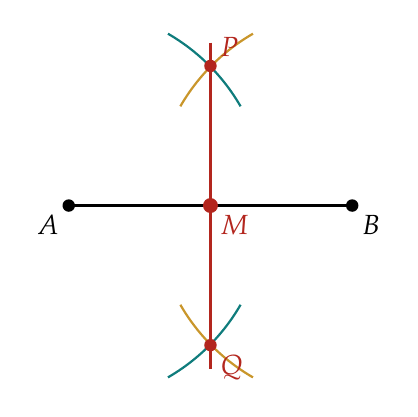
\begin{tikzpicture}[scale=0.9]
\draw[very thick] (0,0)--(4,0); \fill (0,0) circle(2.5pt) node[below left]{$A$} (4,0) circle(2.5pt) node[below right]{$B$};
\onslide<2->{\draw[fteal,thick] (0,0) ++(30:2.8) arc (30:60:2.8); \draw[fteal,thick] (0,0) ++(-30:2.8) arc (-30:-60:2.8);}
\onslide<3->{\draw[fgold,thick] (4,0) ++(150:2.8) arc (150:120:2.8); \draw[fgold,thick] (4,0) ++(-150:2.8) arc (-150:-120:2.8);}
\onslide<4->{\fill[fred] (2,1.97) circle(2.5pt) node[above right]{$P$} (2,-1.97) circle(2.5pt) node[below right]{$Q$};}
\onslide<5->{\draw[fred,very thick] (2,2.3)--(2,-2.3); \fill[fred] (2,0) circle(3pt) node[below right]{$M$};}
\end{tikzpicture}
\end{column}
\begin{column}{0.43\textwidth}
\onslide<2->{\small 1. From $A$: open the compass \textbf{more than half} of $AB$. Arcs above and below.}\par\medskip
\onslide<3->{\small 2. From $B$: the \textbf{same} width. Arcs above and below.}\par\medskip
\onslide<4->{\small 3. The arcs cross at $P$ and $Q$.}\par\medskip
\onslide<5->{\small 4. Line $PQ$ is the \key{perpendicular bisector}. It meets $\overline{AB}$ at the midpoint $M$.}
\end{column}
\end{columns}
\end{frame}

\begin{frame}{Watch out}
\vfill
\warn{Keep the compass width the \textbf{same} for both arcs, and open it to \textbf{more than half} of $AB$ --- otherwise the arcs won't cross.}
\vfill
\end{frame}

\begin{frame}{Bisect an angle}
\begin{columns}[c]
\begin{column}{0.55\textwidth}\centering
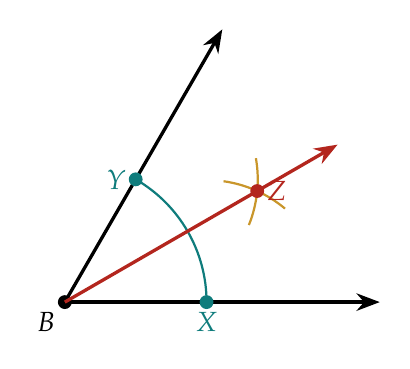
\begin{tikzpicture}[scale=1]
\draw[very thick,-{Stealth}] (0,0)--(4,0); \draw[very thick,-{Stealth}] (0,0)--(60:4); \fill (0,0) circle(2.5pt) node[below left]{$B$};
\onslide<2->{\draw[fteal,thick] (1.8,0) arc (0:60:1.8); \fill[fteal] (1.8,0) circle(2.5pt) node[below]{$X$} (60:1.8) circle(2.5pt) node[left]{$Y$};}
\onslide<3->{\draw[fgold,thick] (1.8,0) ++(50:1.55) arc (50:82:1.55); \draw[fgold,thick] (60:1.8) ++(-22:1.55) arc (-22:10:1.55); \fill[fred] (30:2.821) circle(2.5pt) node[right]{$Z$};}
\onslide<4->{\draw[fred,very thick,-{Stealth}] (0,0)--(30:4);}
\end{tikzpicture}
\end{column}
\begin{column}{0.43\textwidth}
\onslide<2->{\small 1. Arc from the vertex $B$ crosses both sides at $X$ and $Y$.}\par\medskip
\onslide<3->{\small 2. Same width from $X$ and from $Y$: the arcs meet at $Z$.}\par\medskip
\onslide<4->{\small 3. Ray $BZ$ \key{bisects} the angle: two equal halves.}
\end{column}
\end{columns}
\end{frame}

\begin{frame}{Copy a segment}
\begin{columns}[c]
\begin{column}{0.5\textwidth}\centering
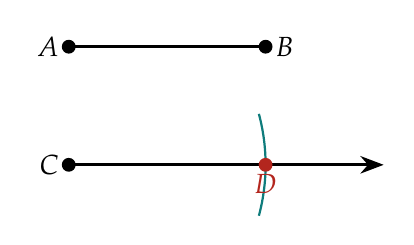
\begin{tikzpicture}
\draw[very thick] (0,1.5)--(2.5,1.5); \fill (0,1.5) circle(2.5pt) node[left]{$A$} (2.5,1.5) circle(2.5pt) node[right]{$B$};
\draw[very thick,-{Stealth}] (0,0)--(4,0); \fill (0,0) circle(2.5pt) node[left]{$C$};
\draw[fteal,thick] (0,0) ++(-15:2.5) arc (-15:15:2.5); \fill[fred] (2.5,0) circle(2.5pt) node[below]{$D$};
\end{tikzpicture}
\end{column}
\begin{column}{0.48\textwidth}\small
Set the compass to $AB$. Put the point on $C$ and draw an arc across the ray. Where it crosses is $D$.\par\medskip
Now $CD = AB$ --- copied without measuring.
\end{column}
\end{columns}
\end{frame}

\begin{frame}{}
\begin{yourturn}
You want to bisect a segment that is $8$ cm long.\par\smallskip
Which compass width works: $3$ cm or $5$ cm?
\end{yourturn}
\pause\bigskip
$\ans{5\text{ cm}}$ --- it must be \textbf{more than half} of $8$ cm, which is $4$ cm.\par\smallskip
{\small\color{gray} With $3$ cm the arcs from $A$ and $B$ never meet.}
\end{frame}

\closeframe{\begin{itemize}\setlength\itemsep{8pt}
\item Only a \key{compass} and a \key{straightedge} --- no measuring.
\item Bisect a segment: same width, more than half, from both ends.
\item The line through the crossings is the \key{perpendicular bisector}.
\end{itemize}}
\end{document}
